\section{SS track identification using a BDT}

To identify tracks that belong to the SS fragmentation, a BDT is trained on simulated LHCb data of the year 2016.
The data includes all tracks in the underlying event of $B_d \rightarrow J/\psi + K*$ and $B_s \rightarrow D_s + \pi$ signal decays.
The BDT input are the 21 features listed in \autoref{tab:SS_features}.
The BDT output resembles a probability of the track being in the SS and is from now on called $\text{Prob}_\text{SS}$.

\begin{table}
    \centering
    \caption{List of all features used in the BDT for SS classification.}
    \label{tab:SS_features}
    \begin{tabular}{c c}
        \toprule
        feature & description \\
        \midrule
        Tr\_p\_proj &  \\
        Tr\_diff\_pt &  \\
        Tr\_diff\_z &  \\
        Tr\_diff\_eta &  \\
        Tr\_cos\_diff\_phi &  \\
        Tr\_T\_AALLSAMEBPV &  \\
        Tr\_T\_BPVIP &  \\
        Tr\_T\_BPVIPCHI2 &  \\
        Tr\_T\_MinIP &  \\
        Tr\_T\_ConIso\_p\_ult &  \\
        Tr\_T\_IPCHI2\_trMother &  \\
        \bottomrule
    \end{tabular}
    \begin{tabular}{c c}
        \toprule
        feature & description \\
        \midrule
        Tr\_T\_IP\_trMother &  \\
        Tr\_T\_IP\_trPUS &  \\
        Tr\_T\_MinBDT\_ult &  \\
        Tr\_T\_Mother\_VtxChi2 &  \\
        Tr\_T\_NbNonIsoTr\_ult &  \\
        Tr\_T\_PT &  \\
        Tr\_T\_SumBDT\_ult &  \\
        Tr\_T\_SumMinBDT\_ult &  \\
        Tr\_T\_Sum\_of\_trackp &  \\
        Tr\_T\_TRGHOSTPROB &  \\
        & \\
        \bottomrule
    \end{tabular}
\end{table}

The implementation of the BDT is done with the Python library XGBoost \cite{xgboost}.
The trained model contains $2000$ estimators at a maximal decision tree depth of $4$.
The learning rate is set to $0.1$.
From the $18$ million tracks, $60\%$ are used for training and $40\%$ are used for validation of the trained model.
Due to the imbalance of SS tracks and other tracks in the data, the parameter \enquote{scale\_pos\_weight} is set to $N_\text{other}/N_\text{SS} = 11.94$.
The learning objective is logistic regression for binary classification.

\begin{figure}
    \centering
    \begin{subfigure}{0.5\textwidth}
        \centering
        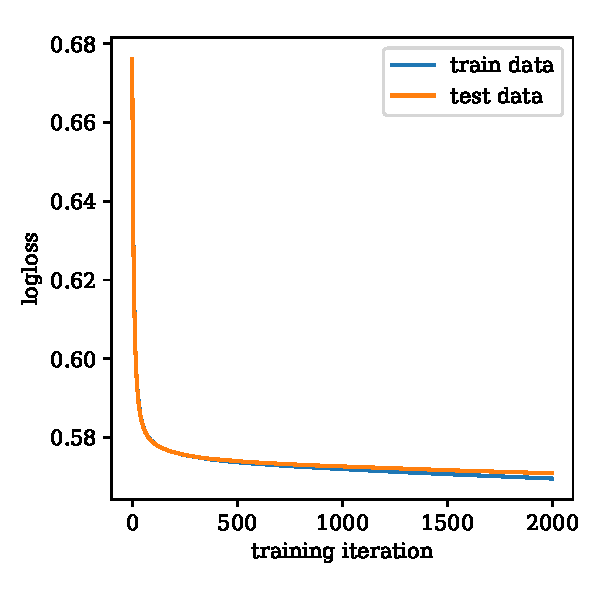
\includegraphics[width=\textwidth]{images/SS_history_logloss.pdf}
        \caption{negative log-likelihood}
    \end{subfigure}%
    \begin{subfigure}{0.5\textwidth}
        \centering
        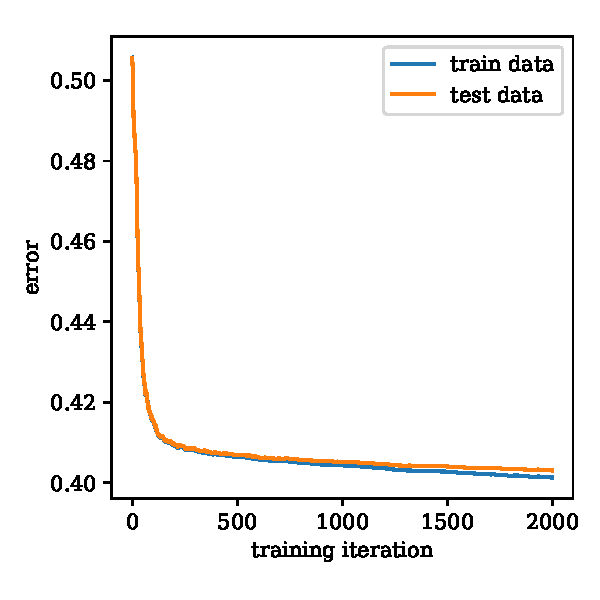
\includegraphics[width=\textwidth]{images/SS_history_error.pdf}
        \caption{error rate}
    \end{subfigure}%
    \caption{Training performance of the SS BDT.}
    \label{fig:SS_history}
\end{figure}

The negative log-likelihood and the error rate for each iteration of the training of the BDT are shown in \autoref{fig:SS_history}.
The error rate is the proportion of predictions matching the simulated ground truth.
For this, all tracks with $\text{Prob}_\text{SS}>0.5$ count as predicted SS tracks. 

To show the achieved separation of the SS tracks, histograms of $\text{Prob}_\text{SS}$ split by the simulation ground truth are shown in \autoref{fig:SS_output}.
A measure of separation is the ROC (reciever operating characteristic) curve shown in \autoref{fig:SS_ROC}.
The achieved ROC AUC (area under the ROC curve) is $0.763$ on the test data and $0.767$ on the training data.
A ROC AUC of $1.0$ means perfect separation and a ROC AUC of $0.5$ means no separation.

To estimate the generalization and overtraining of the model, each performance measure is calculated on both the test data and training data.

\begin{figure}
    \centering
    \begin{subfigure}{0.5\textwidth}
        \centering
        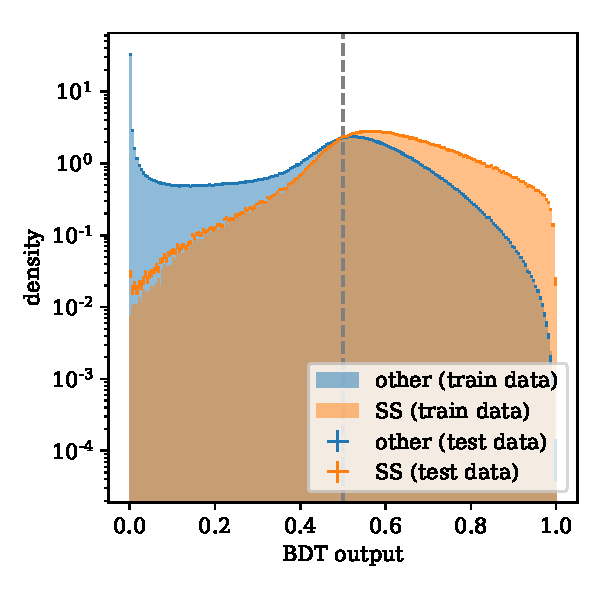
\includegraphics[width=\textwidth]{images/SS_output.pdf}
        \caption{distribution of $\text{Prob}_\text{SS}$}
        \label{fig:SS_output}
    \end{subfigure}%
    \begin{subfigure}{0.5\textwidth}
        \centering
        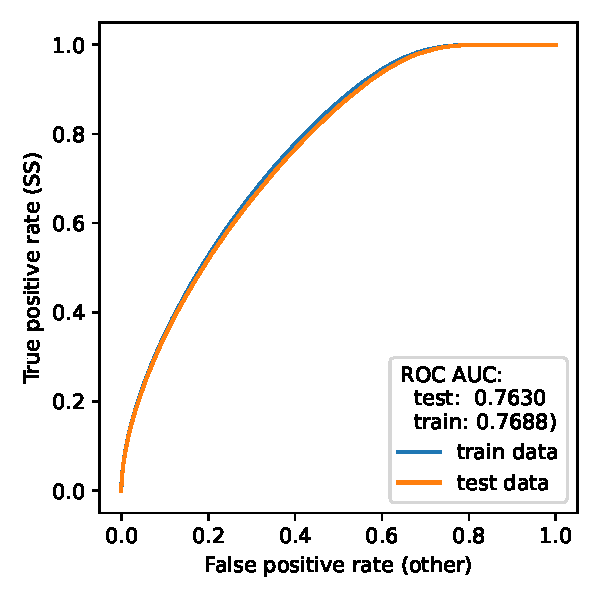
\includegraphics[width=\textwidth]{images/SS_ROC.pdf}
        \caption{ROC curve}
        \label{fig:SS_ROC}
    \end{subfigure}%
    \caption{\autoref{fig:SS_output} shows the distribution of the BDT output split by the simulation ground truth. \autoref{fig:SS_ROC} shows the ROC curve of the BDT output. Both figures show the BDT prediction for the test data and the training data.}
    \label{fig:SS_history}
\end{figure}


